\documentclass[12pt,a4paper]{article}
\usepackage{ctex}
%\usepackage{geometry}
%\bibliographystyle{plain}
\usepackage[super]{gbt7714}
%\geometry{a4paper}
\usepackage[margin=2.3cm]{geometry}
\usepackage{graphicx}
\usepackage{float}%强制左对齐1
\usepackage{longtable}
\usepackage{listings} 
\usepackage{framed}
\usepackage{graphicx}
\graphicspath{{figures/}}
%\usepackage{biblatex}
\usepackage{amsmath}
\usepackage{amsfonts}
\usepackage{xcolor}
\usepackage{soul}
\usepackage{color}
\usepackage{booktabs}



%代码
\lstset{breaklines}  %让LaTeX自动将长的代码行换行排版
\lstset{extendedchars=false}   %这一条命令可以解决代码跨页时,章节标题,页眉等汉字不显示的问题
\lstset{language=C++, %用于设置语言为C++
	identifierstyle=,
	basicstyle=\ttfamily,
	stringstyle=\ttfamily,
	showstringspaces=false,
	frame=shadowbox, %边框
	captionpos=b
}



\title{\heiti 实验六 \quad ENVI区域植被覆盖反演}
\author{}

\date{ }


\newcommand{\upcite}[1]{\textsuperscript{\textsuperscript{\cite{#1}}}} 
\def\degree{${}^{\circ}$}
\definecolor{Seashell}{RGB}{255, 245, 238} %背景色浅一点的
\definecolor{Firebrick4}{RGB}{255, 0, 0}%文字颜色红一点的
\definecolor{shadecolor}{rgb}{0.92,0.92,0.92}%段落背景
\newcommand{\code}[1]{
	\begingroup
	\sethlcolor{Seashell}%背景色
	\textcolor{Firebrick4}{\hl{#1}}%textcolor里面对应文字颜色
	\endgroup
}

\begin{document}
	
	\maketitle	
	\setcounter{page}{45}
	
	\leftline{\textbf{实验时间}:2021年12月5日}	
	\leftline{\textbf{实验环境}:电脑:Windows 10(64 bit); \quad 软件: ENVI 5.3 \quad SP1(64bit)}	
	
	\section{实验要求}
	\begin{enumerate}
		
		\item 
		
		以自己家乡的多幅或一幅Landsat8遥感影像(保证研究区域无云)进行预处理
		
		
		\item 经过裁剪镶嵌和大气校正等处理后,反演近期家乡的植被覆盖度情况
		
		
		\item 掌握图像植被覆盖度反演的计算步骤与方法,并总结方法流程
		
		
		
	\end{enumerate}
	
	\section{实验步骤}
	
	\subsection{对宣城市区域进行大气校正}
	(1)打开上次实验(镶嵌与裁剪)制作的宣城市地区遥感图像,进行快速大气校正,得到校正后的图像\code{QUAC.dat}
	\begin{figure}[H]
		\centering
		\includegraphics[width=.8\textwidth]{air}
	\end{figure}

	\begin{figure}[H]
	\centering
	\begin{minipage}[t]{0.48\textwidth}
		\centering
		\includegraphics[width=5.0cm]{air_1}	
		\caption{QUAC}
	\end{minipage}
	\begin{minipage}[t]{0.48\textwidth}
		\centering 
		\includegraphics[width=5.0cm]{air_11}
		\caption{QUAC相关设置}
	\end{minipage}
\end{figure}

	\begin{figure}[H]
		\centering
		\includegraphics[width=.6\textwidth]{air_12}
		\caption{快速校正后的图像}
	\end{figure}

	\subsection{NDVI计算}
	(1)在ENVI软件界面的右边\code{Spectral}中\code{Vegetation}点击\code{NDVI},文件选用大气校正的图像\code{QUAC.dat}
			\begin{figure}[H]
		\begin{minipage}[t]{0.48\textwidth}
		\centering
		\includegraphics[height=5.0cm]{air_3}	
		\caption{选择NDVI}
	\end{minipage}
	\begin{minipage}[t]{0.48\textwidth}
		\centering 
		\includegraphics[height=5.0cm]{air_31}
		\caption{文件选择}
	\end{minipage}
\end{figure}
(2)然后进入\code{NDVI Calculation Parameters}参数设置界面,文件类型选择\code{Landsat OLI},红光波段设为\code{4},近红光波段选\code{5},最后设置文件保存路径。
\begin{figure}[H]
	\begin{minipage}[t]{0.48\textwidth}
		\centering
		\includegraphics[height=5.0cm]{air_4}	
		\caption{NDVI参数相关设置}
	\end{minipage}
	\begin{minipage}[t]{0.48\textwidth}
		\centering 
		\includegraphics[width=5.0cm]{air_13}
		\caption{计算EDVI}
	\end{minipage}
\end{figure}
(3)得到我们的EDVI图像如下:

	\begin{figure}[H]
	\centering
	\includegraphics[width=.8\textwidth]{NDVI}
	\caption{ENVI计算后的图像}
\end{figure}
\subsection{利用Band Math处理异常数据}

(1)通常我们所认为的\textbf{异常值},是指NDVI指数大于1小于-1的数值,因为根据NDVI定义,NDVI的数值范围应在[-1,1]之间。

$$-1<NDVI<1$$

(2)在ENVI软件界面的右边\code{Toolbox}中点击\code{Band Algebra},然后选择\code{Band Math}。
	\begin{figure}[H]
	\centering
	\includegraphics[height=5cm]{veg_1}
	\caption{选择Band Math
	}
\end{figure}
(3)根据NDVI的性质,我们在\code{Enter an Equation}处输入:
\begin{lstlisting}
	(b1 lt -1)*0+(b1 gt 1)*0+(b1 le 1 and b1 ge -1)*b1
\end{lstlisting}

并将输入的公式进行\code{Add to List}保存。
	\begin{figure}[H]
	\centering
	\includegraphics[height=5cm]{veg_math}
	\caption{输入公式}
\end{figure}
(4)在接下来的页面,选择NDVI的波段数据作为\code{b1}的数据源,并设置保存位置
\begin{figure}[H]
	\centering
	\includegraphics[height=5cm]{veg_pic2}
	\caption{输入公式}
\end{figure}
(5)得到我们的去除异常值的图像。
\begin{figure}[H]
	\centering
	\includegraphics[height=5cm]{veg_qs3}
	\caption{去除异常值的图像}
\end{figure}
\subsection{利用Band Math计算$NDVI_{soil}$和$NDVI_{veg}$}


(1)\textbf{像元二分模型}是一种简单实用的遥感估算模型,它假设一个像元的地表由有植被覆盖部分地表与无植被覆盖部分地表组成,而遥感传感器观测到的光谱信息也由这2个组分因子线性加权合成,各因子的权重是各自的面积在像元中所占的比率,如其中植被覆盖度可以看作是植被的权重。\textbf{当我们的遥感信息为NDVI时},此时我们可以通过利用NDVI信息计算植被的覆盖度。

据此,植被覆盖度的计算公式如下:
$$VFC=\frac{NDVI-NDVI_{soli}}{NDVI_{veg}-NDVI_{soli}}$$

其中,$NDVI$指某一像元点NDVI指数,$NDVI_{soli}$指某一地块裸露土壤NDVI指数,$NDVI_{veg}$指某一地块植被NDVI指数,在这里$NDVI_{soli}$和$NDVI_{veg}$我们通过统计数据来获取。

(2)右键图层管理器的去除异常值的NDVI文件,选择\code{Quick Stats},在[-1,1]之间从选择统计量第一次出现五位数对应的NDVI值设为$NDVI_{soli}$为以及最后一次出现五位数对应的NDVI值设为$NDVI_{veg}$。


\begin{figure}[H]
	\begin{minipage}[t]{0.48\textwidth}
		\centering
		\includegraphics[height=5.0cm]{veg_qs5}	
	
	\end{minipage}
	\begin{minipage}[t]{0.48\textwidth}
		\centering 
		\includegraphics[height=5.0cm]{veg_qs6}
	
	\end{minipage}
\end{figure}




从图中,我们可以确定,$NDVI_{soli}=0.270588$,以及$NDVI_{veg}=0.890196$。

\subsection{利用Band Math计算植被覆盖率}


(1)在ENVI软件界面的右边\code{Toolbox}中点击\code{Band Algebra},然后选择\code{Band Math}。

\begin{figure}[H]
	\centering
	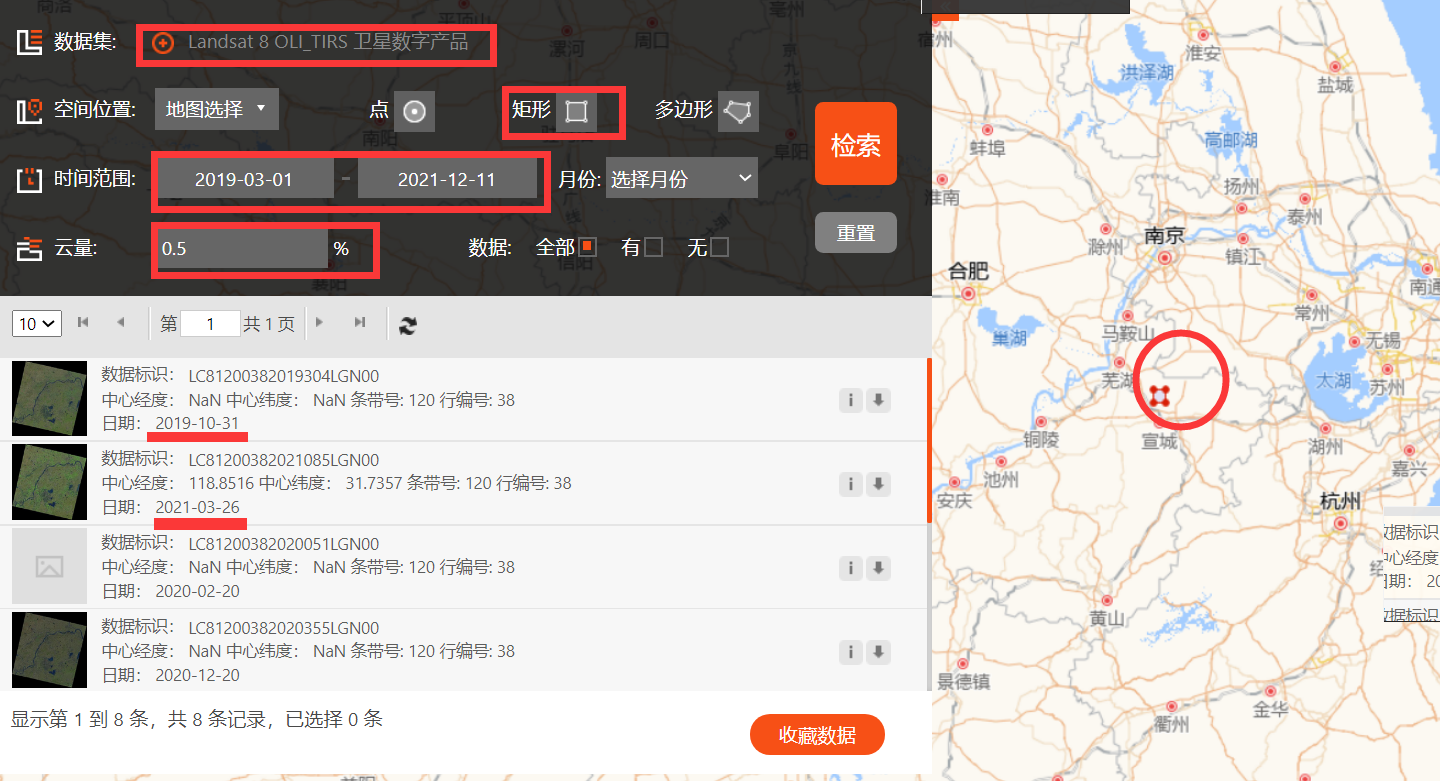
\includegraphics[height=5cm]{1}
\end{figure}

(2)在公式行输入:
\begin{lstlisting}
(b1-0.270588)/ (0.890196-0.270588)
\end{lstlisting}
并选定数据源,仍然是去除异常值的含有NDVI指数文件,最后设置文件保存路径。
\begin{figure}[H]
	\begin{minipage}[t]{0.48\textwidth}
		\centering
		\includegraphics[height=5.0cm]{veg_qs7}	
		\caption{NDVI参数相关设置}
	\end{minipage}
	\begin{minipage}[t]{0.48\textwidth}
		\centering 
		\includegraphics[width=5.0cm]{veg_qs8}
		\caption{计算EDVI}
	\end{minipage}
\end{figure}
(3)得到VFC植被覆盖度的图像如下:

	\begin{figure}[H]
	\centering
	\includegraphics[width=.8\textwidth]{veg_qs9}
	\caption{VFC植被覆盖度图像}
\end{figure}





\end{document}